% ---
% school: "college"
% level: "8eme"
% section: null
% chapter: "التناظر المركزي"
% source: "Axiomaths"
% title: "دائرتان متناظرتان"
% country: "Tunisie"
% year: 2026
% professor: "Axiomaths"
% difficulty: "Moyen"
% points: null
% tags: ["symetrie-centrale", "cercles", "losange", "mediane"]
% ---
% Exercice 12/19 de la série 8ème « التناظر المركزي » (statement + \axsol + solution). Compiler avec XeLaTeX + axiomath.sty (+ axiomaths-logo.png).
\documentclass[12pt,a4paper]{article}
\usepackage[level=8b,color=15803D]{axiomath}
\usetikzlibrary{arrows.meta}
\newcommand{\cm}{\,\mathrm{cm}}
\axsetup{title={التناظر المركزي}, corrige}

\begin{document}

\begin{corr}[title={دائرتان متناظرتان}, stars=3, source={Axiomaths}]
$I$ و $I'$ نقطتان حيث $II'=4\cm$ و $O$ منتصف $[II']$. $\mathcal{C}$ دائرة مركزها $I$ وشعاعها $3\cm$ ، و $\mathcal{C}'$ مناظرتها بالنسبة إلى $O$.
\begin{enumerate}
  \item ابنِ الشكل. بين أن $\mathcal{C}'$ دائرة مركزها $I'$ وشعاعها $3\cm$.
  \item الدائرتان $\mathcal{C}$ و $\mathcal{C}'$ تتقاطعان في نقطتين $M$ و $N$. بين أن $N$ مناظرة $M$ بالنسبة إلى $O$.
  \item بين أن $IMI'N$ معين.
  \item بين أن $(MN)$ عمودي على $(II')$.
\end{enumerate}
\axsol
\begin{enumerate}[itemsep=14pt]
  \item $O$ منتصف $[II']$ ، إذن $I'=S_O(I)$. ومناظرة دائرة مركزها $I$ وشعاعها $3\cm$ هي دائرة مركزها $S_O(I)=I'$ وشعاعها $3\cm$.
  \begin{center}
  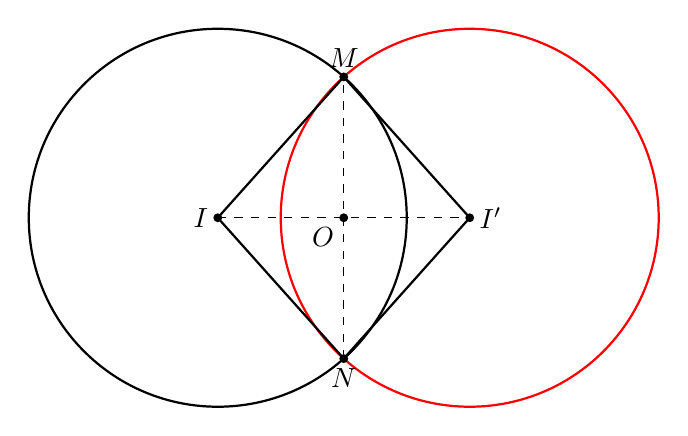
\begin{tikzpicture}[scale=0.8]
    \draw[thick] (0,0) circle (3);
    \draw[thick,red] (4,0) circle (3);
    \draw[dashed] (0,0)--(4,0);
    \draw[dashed] (2,-2.236)--(2,2.236);
    \draw[thick] (0,0)--(2,2.236)--(4,0)--(2,-2.236)--cycle;
    \fill (0,0) circle (2pt) node[left] {$I$};
    \fill (4,0) circle (2pt) node[right] {$I'$};
    \fill (2,0) circle (2pt) node[below left] {$O$};
    \fill (2,2.236) circle (2pt) node[above] {$M$};
    \fill (2,-2.236) circle (2pt) node[below] {$N$};
  \end{tikzpicture}
  \end{center}
  \item $M$ تنتمي إلى $\mathcal{C}$ و $\mathcal{C}'$. بما أن $M\in\mathcal{C}'$ فإن $S_O(M)$ تنتمي إلى $S_O(\mathcal{C}')=\mathcal{C}$ ؛ وبما أن $M\in\mathcal{C}$ فإن $S_O(M)\in S_O(\mathcal{C})=\mathcal{C}'$.
  إذن $S_O(M)$ تنتمي إلى $\mathcal{C}\cap\mathcal{C}'=\{M,N\}$.
  لكن $S_O(M)\neq M$ لأن $M\neq O$ (إذ $OI=2\cm<3\cm$ فالنقطة $O$ داخل $\mathcal{C}$ وليست عليها). إذن \ib{$S_O(M)=N$}.
  \item $IM=3\cm$ لأن $M\in\mathcal{C}$ ، و $I'M=3\cm$ لأن $M\in\mathcal{C}'$. وبالمثل $IN=I'N=3\cm$. إذن
  \[IM=MI'=I'N=NI=3\cm\]
  الرباعي $IMI'N$ أضلاعه الأربعة متقايسة : إنه \ib{معين}.
  \item المثلث $IMI'$ متقايس الضلعين رأسه $M$ ، و $O$ منتصف قاعدته $[II']$ ، فالمستقيم $(MO)$ عمودي على $(II')$. ولأن $O$ منتصف $[MN]$ فإن $N\in(MO)$ ، إذن $(MN)\perp(II')$.
\end{enumerate}
\end{corr}

\end{document}
